\chapter{Collaborative Response to the Opioid Overdose Crisis: Evidence from a Quasi-Experimental Analysis}

\section{\centering Introduction}
As opioid overdoses have increased exponentially over the past two decades, so too has opioid overdose mortality. There were 47,600 fatal opioid overdoses in 2017 \parencite{wilson_drug_2020}, which led the U.S. Department of Health and Human Services to declare a national public health emergency \parencite{johnson_trump_2017}. More recently, fatal drug overdoses exceeded 100,000 in 2021 and 2022, with opioid use driving approximately 76\%, of which is primarily driven by synthetic opioids \parencite{center_for_disease_control_and_prevention_national_2023}. Although 2023 estimates suggest that drug overdoses declined by 3\%, fatal opioid overdoses involving synthetic opioids (e.g., fentanyl) increased from 74,702 to 76,226 -- a 2\% increase \parencite{center_for_disease_control_and_prevention_us_2024}. These trends have produced a need for effective responses to reduce overdose mortality.

There have been a host of federal, state, and local policies and programs devised to combat the opioid overdose crisis. Over the past two decades various state laws have been implemented to curb rising overdose mortality, including Good Samaritan Laws (GSLs), Naloxone Access Laws (NALs), Prescription Drug Monitoring Programs (PDMPs), among others \parencite{haegerich_evidence_2019}. In 2022, the Biden administration set out to award over \$1.6 billion in grants for investments into programs devised to combat opioid use disorder \parencite{us_department_of_health_and_human_services_biden-harris_2022}. Moreover, in 2023, the FDA approved over-the-counter nonprescription use of intranasal naloxone -- an opioid antagonist that reverses the effects of an opioid overdose \parencite{us_food_and_drug_administration_fda_2023}. Additionally, locally, one of the increasingly popular approaches to address the opioid overdose crisis involves collaboration among public safety and public health agencies to make treatment options more accessible for those with OUD \parencite{yatsco_developing_2020}. 

The collaborative efforts between public safety and public health agencies are described as "police-led partnerships" which typically rely on law enforcement officers' (LEOs) unique position in society where they are frequently interacting with people who use opioids (PWUOs). This positions LEOs to be a part of a proactive effort in referring or in some cases, diverting, individuals who have overdosed to social services. Sometimes police contact is followed up by post-overdose outreach efforts which provide information about services available to the individual who previously overdosed \parencite{formica_characteristics_2021}. However, while this approach has gained traction, there have only been two evaluations of post-overdose outreach programs \parencite{donnelly_law_2022, xuan_association_2023}. Both of these studies were conducted in the Northeast United States at the county level. The present study seeks to add to the limited body of research in this area and expand on prior work by looking at a city-level intervention in the Southwest United States

The present study is an evaluation of the Tempe-First Responder Opioid Recovery Project (ORP), a collaborative program between the Tempe Police Department and EMPACT La Frontera (social services organization) to address opioid use in Tempe, Arizona. Using a quasi-experimental approach, I investigate the program's impact on opioid overdose calls for service and fatal opioid overdoses in Tempe. 

\section{\centering Literature Review}
\subsection{Police Role in Reducing Overdose Fatalities}

The police have a broad mandate encapsulated by the duty to protect life \parencite{skolnick_above_1993}. This mandate can appear in practice through many different methods. As community problems shift over time, so do the methods that the police use to address them. One notable community problem that arose in the late 1990s and has caused exponential harm since, is the opioid overdose crisis. Because police officers frequently interact with PWUOs, their role in reducing overdose mortality has shifted from strict drug enforcement to incorporating harm-reduction methods \parencite{beckett_uses_2016}.

In an effort to address the harms created of the opioid overdose crisis, police began carrying naloxone, an opioid antagonist that binds to the opioid receptors in the brain and blocks the opioid from binding to those receptors \parencite{lurigio_opioid_2018}. Recent estimates suggest that approximately 82\% of police departments across the U.S. carry naloxone \parencite{ray_national_2023}, which is a substantial increase from 2019 estimates \parencite{quinn_most_2019}. Given that the police are on scene at overdoses first in many cases \parencite{beletsky_police_2011, silverman_harmonizing_2012, white_leveraging_2022}, it is important to consider the utility of police carrying naloxone. 

However, naloxone is a short-term solution to a much more pervasive crisis. It is a harm reduction tool that can saves lives but it does not address underlying drivers of addiction \parencite{goodison_law_2019,  rando_intranasal_2015, rees_little_2019}. More recently, in some jurisdictions the police role in the opioid overdose crisis has become more involved through diversion or referral methods, and in some instances, these approaches entail collaboration with public health agencies in an effort to be proactive and get individuals with OUD information regarding available services. These approaches are largely a product of public health and public safety agencies recognizing the need to approach the crisis in a collaborative manner to focus on treatment as opposed to traditional law enforcement mechanisms (i.e., arrest).

\subsubsection{Police and Public Health Collaboration}

One such collaborative approach is Law Enforcement Assisted Diversion (LEAD). This approach involves a host of local agencies and criminal justice actors, and centers around law enforcement officers offering services to low level offenders (e.g., sex work, violation of drug laws) in lieu of arrest \parencite{national_institute_of_justice_program_2016}. Originally implemented in Seattle in 2011, this approach has expanded to other cities in an effort to limit contact with the criminal Justice system. With police officers having wider discretion to arrest for low-level offenses, the focus of LEAD is to restrict their discretion and promote a path towards behavioral or social services. Evaluations of LEAD suggest that it is an effective program.

In Seattle, the LEAD program was associated with a 57\% decline in felony charges and arrests \parencite{collins_seattles_2017} and that employment and housing were more likely to be attained \parencite{clifasefi_seattles_2017} among the individuals who were diverted. A more recent evaluation of LEAD in San Francisco produced similar findings indicating that there was a lower likelihood of felony and misdemeanor arrest among those who were diverted \parencite{perrone_harm_2022}. Although LEAD is not focused on OUD, the evidence suggests that utilizing police officers' role in society (e.g., broad mandate, gatekeepers of CJS) to divert low-level offenders away from the criminal justice system by creating pathways to behavioral and social services can reduce contact with the criminal justice system and improve employment and housing situations.

The Police Assisted Addiction Recovery Initiative (PAARI) is similar to LEAD because they focus on law enforcement as a mechanism for diversion or referral but within the context of opioid use \parencite{goodison_law_2019}. PAARI programs provide training and resources to police officers which emphasize the use of non-arrest approaches for those with OUD. The goals of PAARI programs are to limit criminal justice system contact and make treatment options more accessible for those with OUD. This approach has gained traction over the years and has been adapted to involve other approaches that do not necessarily solely rely on police referral or diversion. Depending on the jurisdiction, the various approaches -- which will be discussed below -- are ultimately categorized under the umbrella term "police-led partnerships" and have incorporated post-overdose outreach efforts to provide information to those who have previously overdosed.

Police-led partnerships involve collaboration between law enforcement and public health agencies, with the police having an integral role in the process. The specifics of each approach vary from program to program. For instance, \textcite{formica_post_2018} describe four different types of police-led partnerships: (1) \textit{multi-disciplinary team visits}, (2) \textit{police visit with referrals}, (3) \textit{clinician outreach}, and (4) \textit{location-based outreach}. These approaches employ public health and public safety personnel responses (i.e., post-overdose co-response model), police focused visits, public health/social outreach responses, and a site that has resources, information, etc., respectively \parencite{formica_post_2018}. The three former methods represent the rising collaborative approaches between public safety and public health agencies that have been described as promising approaches \parencite{yatsco_developing_2020}. 

A few examples of police-led partnerships include \textcite{botieri_guide_2016}, \textcite{dahlem_beyond_2017}, \textcite{donnelly_law_2022}, and \textcite{yatsco_alternatives_2020}. \textcite{botieri_guide_2016} highlight a multi-disciplinary team which is made up of a police officer and a behavioral health worker. This team conducts a post-overdose outreach within 24-hours of the overdose to discuss treatment options and other resources that are available. Clinician outreach programs often entail police initiating the response, however, they are not a part of the response. \textcite{dahlem_beyond_2017} describe one of these programs in Washentaw County, Michigan. Following a naloxone administration, a police officer on scene will contact a social outreach worker who will then engage in a post-overdose contact with the individual who survived the overdose. This program structure is similar to \textcite{wagner_training_2016} where police officers initiate a clinician based response following an opioid overdose. An example of a police visit with referrals is the HEROES program in Houston, Texas \parencite{yatsco_alternatives_2020}. Following a nonfatal overdose an officer from the Narcotics Unit within the Houston Police Department visits the survivor to provide information on treatment options and other resources that may be of benefit. Likewise, \textcite{donnelly_law_2022} discuss the Hero Help program in New Castle County, Delaware. This program is a hybrid of police referral, diversion, and self-presentation. An officer may refer someone who previously overdosed to treatment, divert someone towards treatment in lieu of arrest, but also, those who would like to enroll in treatment can go to the police department and request information.\footnote{For a more robust review of post-overdose outreach and police-led partnerships see \textcite{bagley_scoping_2019}, \textcite{bailey_scoping_2023}, \textcite{yatsco_developing_2020}.}

Despite the growing popularity of these approaches, there is limited evaluations of the effectiveness of police-led post-overdose outreach efforts \parencite{bailey_scoping_2023, yatsco_developing_2020}. There are two notable empirical papers that estimate program impact. \textcite{xuan_association_2023} conducts a retrospective interrupted time series analysis across 93 Massachusetts municipalities to analyze the effect of post-overdose outreach programs on opioid fatalities and opioid emergency calls for service. They find that over time there was a decrease in the opioid overdose fatality rate, corresponding to a annualized change of -0.43 per 100,000 population. Likewise, the authors find a decrease in the opioid overdose emergency response rate over time, corresponding to a annualized change of -5.14 per 100,000 population. In a separate study, \textcite{donnelly_law_2022} forecast fatal and non-fatal opioid overdoses using a time series modeling approach in New Castle County, Delaware to estimate the impact of the Hero Help Program. They find that monthly observed fatal and non-fatal overdoses were less than the predicted values after the Hero Help program was implemented. Specifically, they found that in the pooled post-intervention period there were 1.85 fewer fatal overdoses and 7.25 fewer non-fatal overdoses per month which equated to a total of 85 fewer fatal and 333 fewer non-fatal overdoses in the post-intervention period. Both of these articles suggest that comprehensive collaborative post-overdose outreach efforts can be effective. Based on this prior work, I hypothesize: 

\begin{flushleft}
\(H1_a\): \textit{Tempe ORP will be associated with a reduction in opioid overdose calls for service.}
\end{flushleft}

\begin{flushleft}
\(H2_a\): \textit{Tempe ORP will be associated with a reduction in fatal opioid overdoses.}
\end{flushleft}

\noindent However, there is a limited body of evidence in this area. The present study seeks to add to this gap in the literature.

\section{\centering Methods}
\subsection{Data}
The data for this study come from three primary sources. Tempe's opioid overdose data is publicly available at the city's open data catalog (see: \href{https://data.tempe.gov/datasets/2daeeafd2741494c8294ca415e5a793e_0/explore?location=33.398962%2C-111.931850%2C11.93}{https://data.tempe.gov}). The data is produced and managed by Tempe Fire and Medical Rescue (TFMR). Importantly, the open data does not indicate fatal versus non-fatal opioid overdoses. Through a contact at TFMR, I was able to obtain data that indicates fatal or non-fatal calls for service to opioid overdoses. Second, Mesa's open data portal contains confirmed opioid overdoses (see: \href{https://data.mesaaz.gov/Fire-and-Medical/Fire-and-Medical-Opioid-Overdose-Incidents/qufy-tzv6/about_data}{https://data.mesaaz.gov}). This data is produced and managed by Mesa Fire and Medical Department (MFMD). Third, I use American Community Survey (ACS) 1-year estimates for the two cities' demographics.

Due to data constraints in obtaining monthly opioid overdose data at the city-level, I opted to use Mesa's open data portal because of the convenience and because it's proximity to Tempe. Other cities in the Phoenix-metro area were considered but data was not available. The CDC provides monthly data, but at county and state levels. Other opioid overdose data repositories that were considered did not have monthly data. This will be discussed further in the discussion section.

\subsection{Dependent Variables}
I use two primary dependent variables in this study: fatal opioid overdoses and opioid overdose calls for service. Both outcomes are transformed into rates per 100k persons.

With respect to the fatal opioid overdose outcome, it is important to note that these numbers are likely lower bound estimates. Both TFMR and MFMD indicate if the incident is fatal or not based on information gathered on scene. For instance, MFMD's final disposition variable distinguishes between the overdose victim being released on scene, transported to the hospital, or dead on arrival. Thus, those who are transported to the hospital and never regain consciousness are not captured in this dataset.

\subsection{Independent Variable}
The primary independent variable is the interaction of treatment group status in the post-intervention period. Specifically, this interaction captures the effect of the intervention on the treatment group over time, compared to the comparison group. This models the slope change in Tempe compared to Mesa. This estimate is captured by \(\beta_6\) in the equations below.

\subsection{Analytical Sample}
The final sample includes 42 months of data for both Tempe and Mesa which spans from May 2018 to October 2021 (i.e., 84 city-month observations). Thus for both cities, there are 42 pre-intervention observations and 42 post-intervention observations. One-year ACS estimates for 2018, 2019, and 2021 are pulled using the \textit{getcensus} command in Stata. Estimates for 2020 were interpolated due to the unavailability of 2020 ACS data \parencite{chamberlain_relative_2016}.

\subsection{Analytical Plan}

To evaluate the impact of the Tempe ORP, I use a Comparative Interrupted Time Series Design (CITS). This approach is employed for a few reasons. First, the interrupted time series design is a popular quasi-experimental modeling technique that has been used to evaluate policy interventions in a variety disciplines including public health, epidemiology, and criminal justice. Moreover, the CITS design is particularly strong due to its ability to account for time-varying confounders \parencite{lopez_bernal_use_2018}. Second, this design accounts for the baseline mean and trend of the outcome variable over time. Third, like a difference-in-differences (DiD) model, equivalence between the treatment and comparison groups is not needed \parencite{anglin_validity_2023}. The counterfactual in a CITS design is constructed by assuming that the pre-to-post change in the intercept and slope in the comparison group could be imputed into the treatment group, absent the intervention. Whereas the DiD counterfactual is constructed focusing on the average outcome. Namely, the pre-to-post change in the average outcome in the treatment group would have been similar to the comparison group in the absence of the intervention. Although the construction of the counterfactual is different for these two models, they have been shown to produce similar estimates \parencite{anglin_validity_2023, somers_validity_2013}. 

I use Mesa as a location-based comparison group, which is a city in Arizona that is adjacent to Tempe. The use of Mesa as a comparison group is important for a couple reasons. First, the comparison group improves the rigor of the single-group ITSA (Interrupted Time Series Analysis) by reducing the impact of time-varying confounding variables \parencite{shadish_experimental_2002}. The effects of Covid-19, for instance, began within a month and a half of the start of the program. Thus, a single-group ITSA would be limited in providing reliable estimates of program impact. Second, state-level or county-level exogenous shocks are less likely to be a confounder given that both Tempe and Mesa are in the same county in Arizona.

\subsubsection{Interrupted Time Series Analysis}

Single-group Interrupted Time Series Model:
\[Y = \beta_0 + \beta_1 T + \beta_2 POST + \beta_3 TS + \epsilon \]

Where \(Y\) is the outcome of interest (opioid overdose calls for service rate and opioid overdose fatality rate per 100,000). \(\beta_0\) is the intercept of outcome \(Y\). \(\beta_1\) is the coefficient for time in months over the course of the study period. \(\beta_2\) represents the coefficient for the treatment period (= 1 if in the post-treatment period [0 = pre-intervention]). \(\beta_3\) is the coefficient for time since the intervention (\(t\)= 1, 2, 3 ... \(T\) for months after treatment).

Comparative Interrupted Time Series Model:
\[Y = \beta_0 + \beta_1 T + \beta_2 TX + \beta_3 TXT + \beta_4 POST + \beta_5 TXPOST + \beta_6 TS + \beta_7 TXTS + \epsilon \]

Where \(Y\) is the outcome of interest (Opioid overdose calls for service rate and opioid overdose fatality rate per 100,000). \(\beta_0\) is the intercept of outcome \(Y\). \(\beta_1\) represents the coefficient for time, which is a continuous measure. \(\beta_2\) is the coefficient for a treatment variable (= 1 if group is in the treatment group [0 = control]). \(\beta_3\) corresponds to the coefficient of an interaction between the treatment assignment and time. \(\beta_4\) is the coefficient for the post-intervention period (= 1 if in the post-treatment time period [0 = pre-intervention]). \(\beta_5\) coefficient corresponds to an interaction between the treatment and post-intervention variable. \(\beta_6\) is the coefficient for time since the intervention (\(t\)= 1, 2, 3 ... \(T\) for months after treatment). Lastly, the \(\beta_7\) is the interaction between treatment assignment and time since intervention. Error is captured by \(\epsilon\).

The above regression models are estimated in Stata \parencite{statacorp_stata_2023} using the \textit{itsa} command. Autocorrelation is accounted for with the use of Newey-West standard errors with a maximum lag of 1 (see Appendix C.2).

\section{\centering Results}
Table 5 provides the characteristics of each city by year. Tempe has just over a third of the population of Mesa. Tempe has a lower proportion of White residents although both cities experience a decline in the percentage of White residents over time. There is a similar trend regarding the proportion of Hispanic residents. There is a higher proportion of Black residents in Tempe, and similar to above, there is a decline in the proportion of Black residents in both cities. The percent of the population below poverty is higher in Tempe with a small decline over time and a somewhat more pronounced decline in Mesa. Tempe has a higher proportion of residents aged 20-24 and 25-34. Moreover, it has a higher proportion of residents with a Bachelor's degree. The median household income is fairly similar and increases over time for each city. Notably, there are differences between Tempe and Mesa but for many of the characteristics, they trend similarly over time. 

Figure 2 provides a visualization of trends for opioid overdose calls for service, non-fatal opioid overdoses, and fatal opioid overdoses in Tempe and Mesa. The rate of opioid overdose calls for service trend similarly in the pre-intervention phase for both Tempe and Mesa, although in November 2019, Mesa had a sharp increase in calls for service and fatal overdoses (Panels A and C). Calls for service to opioid overdoses almost doubled from October (69; 13.3 per 100k) to November (122; 23.6 per 100k) with the fatality rate increasing from 1.4 per 100k to 7.1 per 100k. In the adjusted CITS model below, this outlier is controlled for (also see Appendix C.3).

Table 6 shows the results from the single-group time series models. There is no indication that the treatment is significantly associated with either of the outcomes. Although, there is a non-significant decline in the slope for opioid overdose calls for service and fatal opioid overdoses in the post-intervention period. Additionally, the post-period variable indicates the immediate impact of the intervention (e.g., non-signifcant increase), and the linear time trend variable suggests that opioid overdose calls for service and fatal opioid overdoses increased over time during the pre-intervention period, albeit non-significantly. 

The CITS models comparing Tempe and Mesa are presented in table 7. The main coefficient of interest is the 'treatment x time since treatment' variable. This captures the trend of the outcome for the treatment group since the intervention compared to the trend of the comparison group. Focusing on this variable, none of the models suggest there is a treatment effect for the rate of opioid overdose calls for service or fatal overdoses (model 1: \(b\) = 0.169 [-0.297, 0.635]; model 2: \(b\) = 0.126 [-0.052, 0.305]; model 3: \(b\) = 0.066 [-0.070, 0.201]; see figures 3 and 4 for a visualization).  

\section{\centering Discussion}
% contextualize
The present study uses a non-equivalent comparison group in a CITS design to evaluate the impact of the Tempe ORP. When comparing Tempe to Mesa, the findings suggest that the Tempe ORP did not significantly impact rates of opioid overdose calls for service or fatal opioid overdoses. The results do not support the hypothesized relationships. 

Prior studies that have evaluated the effectiveness of collaborative post-overdose outreach programs have produced findings that indicate their effectiveness. \textcite{donnelly_law_2022} look at New Castle County of Police and use an Autoregressive Integrated Moving Average model to forecast the counterfactual in the post-intervention period. They compare this with the observed number of opioid overdoses and fatal opioid overdoses. Additionally, \textcite{xuan_association_2023} compare counties that adopted the post-overdose outreach program to those that did not in Massachusetts. Similar to the approach in the present study, the authors use a comparative interrupted time series design. Both of the above studies find that the collaborative post-overdose outreach efforts were associated with reductions in fatal opioid overdoses, while \textcite{donnelly_law_2022} report a decline in opioid overdoses, and \textcite{xuan_association_2023} report a decline in the EMS response rate to opioid overdoses. 

There are some qualitative and quantitative differences between the current study and the prior studies discussed above. Both of the above studies were conducted in the Northeastern United States at the county level, whereas the present study was conducted in Arizona at the city level. Moreover, the specifics of each program differ. For instance, the Hero Help program evaluated by \textcite{donnelly_law_2022} focuses on deflection. Specifically, individuals can ask for help, officers can recommend entering the program, or the officer can divert individuals into the program as an alternative to criminal charges. The program incorporated a community based deflection pathway as well by focusing on sharing information about the program. \textcite{xuan_association_2023}'s analysis evaluates a host of different collaborative post-overdose outreach efforts across counties in Massachusetts. The authors acknowledge that many of the programs are similar but there is variation across counties (see Formica et al., 2021). The Tempe ORP does not have this level of variation in program efforts like \textcite{xuan_association_2023} describe. Additionally, in contrast to \textcite{donnelly_law_2022}'s evaluation of the Hero Help program, the Tempe ORP does not focus on deflection. Police officers initiate the post-overdose outreach by being on scene at an overdose and calling a 24-hour hotline that then relays information about the individual and the overdose to a peer navigator. Once this call is made, the situation is then in the hands of the peer navigator from EMPACT. 

Quantitatively, the present study utilizes a comparative interrupted time series design. This builds upon the single-group analysis conducted by \textcite{donnelly_law_2022}. However, in contrast to \textcite{xuan_association_2023}, the current study uses just one comparison group which hinders the study's power. Additionally, both prior studies have many months of data, particularly for the pre-intervention period which improves the models' ability to accurately capture trends and develop more accurate counterfactuals. \textcite{donnelly_law_2022} use data from January 2013 through December 2021, with March 2018 and December 2020 being inflection points. \textcite{xuan_association_2023} use data from January 2013 through June 2019. For the counties in their study, the adoption of post-overdose outreach efforts varied across time.

% interpret
Further contextualizing the current study, COVID-19 and the ensuing governmental restrictions took place approximately a month and a half after the first Tempe police officer administered naloxone. Although the use of a comparison group helps control for this time-varying confounder, COVID-19 altered the peer-navigator's ability to contact opioid overdose victims. For instance, the post-overdose outreach to the hospital became more difficult as hospitals began to enforce restrictions on how many people and who could enter the emergency room. Tempe PD and EMPACT had to alter their practices and develop a co-response model to get peer-navigators in to see overdose victims. This period of reforming the approach could have impacted engagement rates with services. Although, the project has generally maintained high engagement rates over the course of the project \parencite{watts_tempe_2023}.

Additionally, Mesa is adjacent to Tempe and this proximity to the treatment area creates the potential for spillover effects -- a potential SUTVA violation \parencite{rubin_formal_1990}. There is one primary way this is possible: contact with the peer-navigator following an overdose, with two potential underlying mechanisms. \textit{Mechanism 1}: A Mesa resident overdoses in Tempe, is contacted by the post-overdose outreach peer navigator, and then engages in services. Accepting services could contribute to decline in opioid use or riskier use, and thus, fatal opioid overdoses in Mesa. \textit{Mechanism 2}: After being contacted by the post-overdose outreach peer navigator, naloxone is provided to the individual and/or friends and family of the individual. This could impact Mesa's calls for service to overdoses and fatal overdoses as well. Prior research has highlighted naloxone's effectiveness at reversing opioid overdoses \parencite{giglio_effectiveness_2015}. Because of its effectiveness, there is a potential subset of opioid overdose incidents that are not reported because a layperson's administration of naloxone reverses the effects of an opioid overdose. 

Further, through personal communication with the primary peer-navigator at EMPACT, he noted that it was common for the post-overdose outreach efforts to be for someone who had an address (or last known address) in an adjacent city to Tempe -- Phoenix, Mesa, and Gilbert, for instance \parencite{watts_personal_2024}. Although, the frequency with which this occurred specifically for Mesa is not clear.

\subsection{Limitations}
There are some limitations to discuss. First, one city is used as a comparison group. Mesa was the only city in Arizona to have open data available. Given the data constraints faced, this was the most sound analytical approach available. Nonetheless, a sample size of two cities hinders the power of the study. Second, Mesa is a non-equivalent comparison group. Because they are non-equivalent, selection bias is a concern that is not overcome in the present study. Third, the significant outlier in the pre-intervention phase for Mesa does cause some concern regarding the reliability of the data and its use as a comparison group.\footnote{I contacted the manager of the dataset in Mesa to ask about the increase in November 2019 to hopefully get some context. I did not receive a response. Moreover, I searched for local news articles discussing a rise in opioid overdoses or articles discussing a rise in seizures of fentanyl. I did not find any news articles to contextualize the outlier.} Lastly, as mentioned above, there is a potential SUTVA violation. Overcoming this issue would require adequate comparison group(s) be used that are unlikely to have come in contact with a peer-navigator from EMPACT. Unfortunately, the availability of this data is lacking.

\subsection{Implications}
Given the economic and social costs of the opioid overdose crisis, it is paramount that local trends in fatal and nonfatal opioid overdoses be analyzed. This is not a new call for improvements in the availability of data, many have discussed the lack of data available to understand opioid overdose trends in real time and the need to revamp the data collection and dissemination process \parencite{blanco_data_2022, volkow_need_2022}. Despite these calls, opioid data infrastructure still lacks. The current study highlights that there are city-level interventions that ought to be evaluated to determine their impact on opioid opioid overdoses. Currently, however, the ability to employ robust quasi-experimental designs is limited because of the lack of data at the city-level. 

The largest city-level data repository is hosted at Drexel University, with only yearly estimates available.\footnote{\url{https://drexel.edu/uhc/research/projects/BCHI/Drug\%20Overdose\%20Deaths\%20in\%20Big\%20Cities/}} This is a great source for analyzing year-to-year trends in a select subset of cities across the country. However, it is focused on large cities and does not provide data at a more granular level (e.g., monthly). The CDC provide county and state fatal opioid overdose data which can be downloaded at weekly, monthly or yearly increments. This is a great source for evaluating macro-level interventions but lacks in timeliness and availability at more granular geographic areas (e.g., cities). Moreover, the Overdose Detection Mapping Application Program (ODMAP) combines law enforcement, emergency medical services, and other health related data in near real time to provide a comprehensive data repository. However, the data is only available to governmental agencies \parencite{blanco_data_2022}

Inter-agency collaboration is a key step in developing comprehensive datasets that are timely and can be analyzed at various geographic levels. For instance Massachusetts Department of Public Health has developed a comprehensive collaborative approach to collecting and disseminating data for awareness campaigns, policymakers, and clinicians \parencite{bharel_using_2020}. Moreover, with the proliferation of artificial intelligence and large language models, data collection and management could be less time consuming and may enable data linkage across departments in a much more efficient way. 

\section{\centering Conclusion}
The current study suggests that in the aggregate, the Tempe ORP did not lead to a reduction in opioid overdose calls for service or fatal opioid overdoses. There are a few explanations for why this may be the case which include methodological and data constraints, COVID-19, and potential SUTVA violation. 

Data collection, management, and dissemination practices must improve to facilitate timely and rigorous evaluations of city-wide interventions. Improvements in these areas can help limit the methodological constraints that researchers face. Indeed, comprehensive city-level data availability could facilitate robust quasi-experimental methods to better understand city-level interventions which would ideally lead to more effective policies and programs being implemented. Without this data, it is difficult -- if not impossible -- to produce reliable estimates of treatment effects.

Despite the methodological issues, the Tempe ORP has produced meaningful findings over the last four years. First, Tempe police officers did not have naloxone prior to the intervention. Since February 2020, Tempe police officers responded to more than 323 suspected opioid overdose incidents.\footnote{This is the most recent estimate from November, 2023.} Of the 323 overdose incidents, 294 resulted in a positive response to the naloxone dose(s) and the individuals recovered (91\%). Second, EMPACT's engagement rate with overdose survivors has been higher than prior work in this space. Prior studies have noted engagement rates of approximately 25\%, whereas the Tempe ORP has steadily been around 50\% \parencite{dahlem_beyond_2017, wagner_training_2016, watts_tempe_2023, white_moving_2021}. These are meaningful outcomes that indicate program success. 

Collaborative post-overdose outreach is an innovative way to reach PWUOs and provide resources to them. Prior evaluative work indicates that post-overdose outreach programs can reduce opioid overdoses and fatal opioid overdoses. The present study casts some doubt on the effectiveness of this approach. Nonetheless, this is still a small body of research that have applied varying methodological approaches. More evaluation work is needed in this area. 

\pagebreak

\begin{table}[htbp]\centering
\def\sym#1{\ifmmode^{#1}\else\(^{#1}\)\fi}
\caption{\centering Summary Statistics by City and Year}
\begin{adjustbox}{max width=\linewidth}\begin{tabular}{l*{4}{c}}
\toprule
                    &        2018&        2019&        2020&        2021\\
\midrule
\textbf{Mesa}                &            &            &            &            \\
Fatal opioid overdose rate per 100k&        1.08&        1.98&        3.14&        2.78\\
Opioid overdose calls for service rate per 100k&        9.28&       12.31&       17.04&       19.72\\
Population          &   508979.00&   517981.00&   504258.00&   509492.00\\
Median household income&    58247.00&    63836.00&    66551.00&    69266.00\\
\% Bachelor's degree or higher (25 years +)&       26.90&       29.20&       30.75&       32.30\\
\% Aged 20-24       &        6.50&        6.50&        6.35&        6.20\\
\% Aged 25-34       &       15.30&       15.50&       15.20&       14.90\\
\% White            &       81.00&       81.40&       73.40&       65.40\\
\% Black            &        5.00&        5.60&        4.75&        3.90\\
\% Hispanic         &       24.00&       22.50&       22.35&       22.20\\
\% Below poverty    &       13.90&       11.60&       10.85&       10.10\\
\midrule
\textbf{Tempe}               &            &            &            &            \\
Fatal opioid overdose rate per 100k&        1.04&        0.77&        1.43&        1.14\\
Opioid overdose calls for service rate per 100k&       20.60&       20.09&       23.03&       22.91\\
Population          &   192354.00&   195816.00&   180587.00&   184109.00\\
Median household income&    60330.00&    66297.00&    67479.50&    68662.00\\
\% Bachelor's degree or higher (25 years +)&       47.60&       50.30&       49.70&       49.10\\
\% Aged 20-24       &       17.60&       16.20&       16.55&       16.90\\
\% Aged 25-34       &       21.50&       24.40&       24.35&       24.30\\
\% White            &       68.70&       73.80&       66.95&       60.10\\
\% Black            &        6.60&        7.50&        6.00&        4.50\\
\% Hispanic         &       18.20&       16.70&       17.10&       17.50\\
\% Below poverty    &       17.40&       17.20&       16.95&       16.70\\
\bottomrule
\multicolumn{5}{l}{\footnotesize Means displayed; ACS 1-year estimates; 2020 estimates interpolated.}\\
\end{tabular} \end{adjustbox}
\end{table}


\begin{figure}
    \caption{\centering Opioid Overdose Trends: Tempe and Mesa, Arizona}
    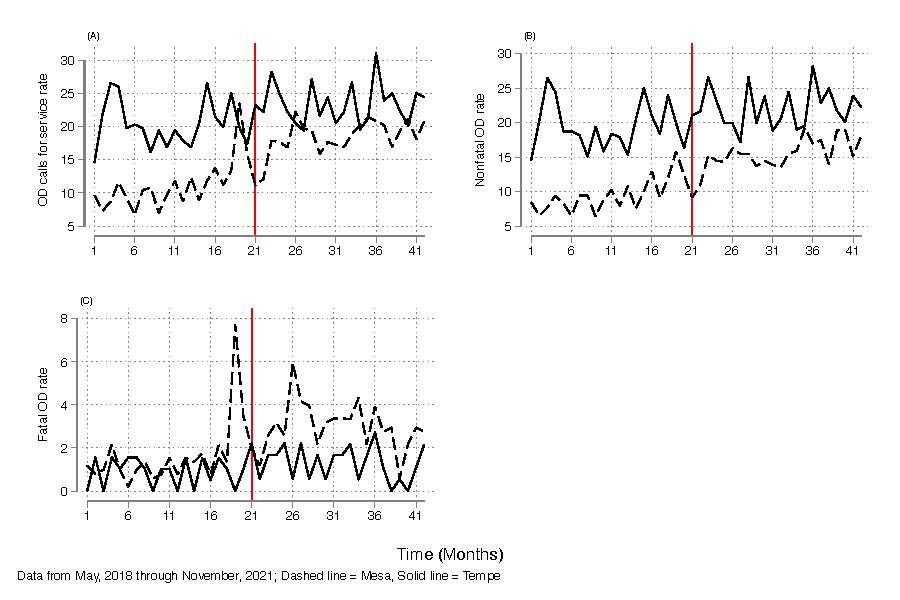
\includegraphics{figures/rates_combined.pdf}
\end{figure}


\begin{table}[htbp]\centering
\def\sym#1{\ifmmode^{#1}\else\(^{#1}\)\fi}
\caption{\centering Single-Group Interrupted Time Series Models}
\begin{tabular}{l*{2}{c}}
\toprule
                &\multicolumn{1}{c}{(1)}&\multicolumn{1}{c}{(2)}\\
                &\multicolumn{1}{c}{OD calls for service rate per 100k}&\multicolumn{1}{c}{Fatal OD rate per 100k}\\
\midrule
Time (months)   &0.039 (0.143)        &0.013 (0.024)        \\
\addlinespace
Post-period     &2.360 (1.969)        &0.379 (0.443)        \\
\addlinespace
Treatment X Post-period&-0.018 (0.175)        &-0.031 (0.036)        \\
\addlinespace
Constant        &20.043\sym{**} (1.810)        &0.809\sym{**} (0.243)        \\
\midrule
Observations    &       42        &       42        \\
F-statistic     &    2.914        &    1.908        \\
\bottomrule
\multicolumn{3}{l}{\footnotesize Newey-West standard errors (AR 1) in model 2}\\
\multicolumn{3}{l}{\footnotesize \sym{*} \(p<0.05\), \sym{**} \(p<0.01\), \sym{**} \(p<0.001\)}\\
\end{tabular}
\end{table}


\begin{table}[htbp]\centering
\def\sym#1{\ifmmode^{#1}\else\(^{#1}\)\fi}
\caption{\centering Comparative Interrupted Time Series Models: Mesa Comparison}
\begin{adjustbox}{max width=\linewidth}\begin{tabular}{l*{3}{D{.}{.}{-1}}}
\toprule
                &\multicolumn{1}{c}{OD calls for service per 100k}&\multicolumn{2}{c}{Fatal OD rate per 100k}\\\cmidrule(lr){2-2}\cmidrule(lr){3-4}
                &\multicolumn{1}{c}{(1)}        &\multicolumn{1}{c}{(2)}        &\multicolumn{1}{c}{(3)}        \\
\midrule
Time (months)   &    0.363\sym{**}&    0.124        &    0.063\sym{*} \\
                &  (0.128)        &  (0.062)        &  (0.028)        \\
\addlinespace
Treatment       &   12.576\sym{**}&    0.407        &    0.077        \\
                &  (2.068)        &  (0.518)        &  (0.372)        \\
\addlinespace
Treatment X Time&   -0.324        &   -0.110        &   -0.050        \\
                &  (0.192)        &  (0.067)        &  (0.037)        \\
\addlinespace
Post-period     &    1.781        &    0.372        &    1.322        \\
                &  (2.223)        &  (1.106)        &  (0.756)        \\
\addlinespace
Treatment X Post-period&   -0.188        &   -0.158        &   -0.097        \\
                &  (0.156)        &  (0.082)        &  (0.058)        \\
\addlinespace
Time since treatment&    0.579        &    0.006        &   -0.943        \\
                &  (2.970)        &  (1.191)        &  (0.878)        \\
\addlinespace
Treatment X Time since treatment&    0.169        &    0.126        &    0.066        \\
                &  (0.234)        &  (0.090)        &  (0.068)        \\
\addlinespace
Mesa outlier    &                 &                 &    5.864\sym{**}\\
                &                 &                 &  (0.292)        \\
\addlinespace
Constant        &    7.466\sym{**}&    0.402        &    0.732\sym{*} \\
                &  (1.001)        &  (0.458)        &  (0.280)        \\
\midrule
Observations    &       84        &       84        &       84        \\
F-statistic     &   49.986        &    9.031        & 1065.290        \\
\bottomrule
\multicolumn{4}{l}{\footnotesize Newey-West standard errors (AR 1) for models 2 and 3}\\
\multicolumn{4}{l}{\footnotesize \sym{*} \(p<0.05\), \sym{**} \(p<0.01\), \sym{**} \(p<0.001\)}\\
\end{tabular} \end{adjustbox}
\end{table}
 

  
\newpage


\begin{figure}
\begin{minipage}{1 \textwidth}
    \centering
    \caption{\centering CITS Visualization}
    \includegraphics{figures/itsa-combined.pdf}
\end{minipage}
\begin{minipage}{1 \textwidth}
    \centering
    \caption{\centering Coefficient Plot}
    \includegraphics{figures/coefplot.pdf}
\end{minipage}
\end{figure}



